\documentclass[a4paper, 12pt, italian]{report}
\usepackage{ctable}
\usepackage{url}
\usepackage[utf8]{inputenc}
\usepackage{graphicx}
\usepackage{amsmath}
\usepackage[italian]{babel}

\begin{document}
\begin{titlepage}
\newcommand{\HRule}{\rule{\linewidth}{0.5mm}} 
\center 
\textsc{\LARGE Università degli studi di Salerno}\\[1cm] 

\includegraphics[width=3.5cm]{img/logo.jpg} \\[1cm]
\textsc{\large Progetto di Ingegneria del Software II}\\[0.5cm]
\textsc{\Large Repominer Evolution}\\[0.5cm] 
 \HRule \\[0.4cm]
{ \large \bfseries Software Project Management Plan}\\[0.4cm] 
\HRule \\[1.5cm]

\begin{minipage}{0.4\textwidth}
\begin{flushleft} \large
\emph{Autori:}\\
Matteo \textsc{Merola}\\
Carlo \textsc{Branca}\\
Simone \textsc{Scalabrino}\\
Giovanni \textsc{Grano}\\
\end{flushleft}
\end{minipage}
~
\begin{minipage}{0.4\textwidth}
\begin{flushright} \large
\emph{Supervisore:} \\
Prof. Andrea \textsc{De Lucia}
\end{flushright}
\end{minipage}\\[2.5cm]

{\Large SPMP}\\
Versione 1.0\\[1cm]

{\large \today} % Date, change the \today to a set date if you want to be precise

\vfill

\end{titlepage}	
	\setcounter{tocdepth}{1}	
	\tableofcontents
	
	\chapter{Introduzione}

\section{Scopo del documento}
		
Il presente documento, oltre a fornire una panoramica del progetto, descrive il processo di management che sarà portato avanti durante le fasi progettazione e sviluppo. Il documento sarà aggiornato in maniera iterativa per offrire informazioni più precise riguardo le diverse fasi del progetto. 


\section{Evoluzione del presente documento}

Allo stato attuale del progetto, molte informazioni nel SPMP risultano incomplete o poco precise. Il documento sarà aggiornato e rivisto con l'avanzare dei lavori in modo da garantire una completa descrizione del processo manageriale condotto.


\section{Definizioni ed acronimi}

Definizioni:			
\begin{itemize}
\item \emph{Deliverables}: con il termine deliverables si ci riferisce generalmente alla documentazione tecnico/commerciale da consegnare al cliente quale risultato dell'esecuzione di una o più fasi di un progetto.
\item \emph{Scheduling}: pianificazione dei tempi e delle precedenze nell'impiego di risorse materiali ed umane per un buon svolgimento del processo di progettazione e sviluppo di un sistema software.
\item \emph{Work breakdown structure (WBS)}: rappresentazione di un progetto che consiste in una strutturazione tipicamente gerarchica delle attività che lo compongono in sotto-attività fino ad un opportuno livello di approfondimento.
\item \emph{Diagramma di Gantt}: strumento di supporto alla gestione dei progetti utilizzato principalmente nell'attività di project management quale rappresentazione dello scheduling delle attività o mansioni che costituiscono un progetto.
\end{itemize}	

Acronimi:
\begin{itemize}
\item \emph{ODD}: Object Design Document
\item \emph{WBS}: Work Breakdown Structure
\end{itemize}
	\chapter{Organizzazione del progetto}	
		
		\section{Organizzazione strutturale}
		\label{sec:struc}
		
		La struttura organizzativa del progetto risulta difficile da stabilire in questa fase preliminare. In fasi più avanzate, i team member potranno essere suddivisi in team dedicati ad attività specifiche (Es. team di implementazione, team di testing).
		
		\begin{figure}[ht]
		\centering
		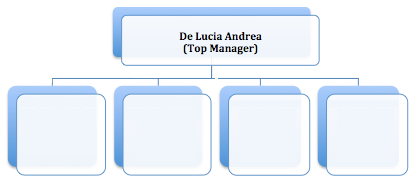
\includegraphics[width=\textwidth]{img/organizzazione.png}
		\caption{Struttura organizzativa}\label{fig:1}
		\end{figure}
		
		\begin{table}[ht]
		\centering
			\begin{tabular}{|c|c|c|}
				\hline
				\textbf{Nome componente} & \textbf{Ruolo} & \textbf{Responsabilità}\\
				\hline
				Matteo Merola & Team member & \shortstack{Sviluppo deliverables:\\DL1, DL2, DL3}\\
				\hline
				Simone Scalabrino & Team member &  \shortstack{Sviluppo deliverables:\\DL1, DL2, DL3}\\
				\hline
				Giovanni Grano & Team member & \shortstack{Sviluppo deliverables:\\DL1, DL2, DL3}\\
				\hline
				Carlo Branca & Team member & \shortstack{Sviluppo deliverables:\\DL1, DL2, DL3}\\
				\hline
			\end{tabular}
		\caption{Ruoli e responsabilità}
		\label{proj_org:ruoli}
		\end {table}
		
	\chapter{Managerial process}
		
		\section{Objectives and priorities}
			
			During the development of the system, the following objectives should be kept
			in mind:
			
			\begin{enumerate}
				
				\item The project should meet the requirements of the customer
				\item Deadlines have to be respected
				\item Reusability and extensibility of the software is very important
				\item The system should be stable
				
			\end{enumerate}	
			
		\section{Assumptions, dependencies and constraints}
			
			\begin{itemize}
				
				\item No assumptions will be made.
				
				\item Dependencies \\
 					  For the project to succeed, it will depend on
					  the knowledge and the motivation of the team members	
				
				\item Constraints:
				\begin{itemize}
					\item Only open-source software is to be used
					\item The product should run in a Linux environment
					\item The product should run on the Wilma server
				\end{itemize}
				
			\end{itemize}	
			
		\section{Risk Management}
			
			Developing software introduces a lot of risks. At regular times these risks will
			be discussed in order to reduce or eliminate them. Each member is encouraged to report
			possible risk to the project leader.
			
			\subsection{Google goes down for a certain period}
			\textbf{Criticality}: + \\
			We need to make backups of our files and documentation. This will be 
			performed by the configuration team.
			
			
			\subsection{Lack of knowledge of certain tools or mechanisms}
			\textbf{Criticality}: ++++ \\
			Some tools and mechanisms will be completely new to some team members which can
			results in a lack of knowledge and inefficiency. Initially, tutorials will be made
		    as Wiki-pages. Ultimately presentations can be given if the subject is too complex or
		 	if it demands a complete explanation. 
			
			\subsection{Somebody becomes ill}
			\textbf{Criticality}: +++ \\
			This risk has already been considered in the beginning of this 
			project. This is why there is an Assistant(formerly called Backup) for 
			every Management position. If a leader or manager gets ill, the assistant 
			of that function should be able to fully understand his 
			function and replace that leader or manager, for a certain period of time.
			
			\subsection{Risk Table}
			The above risks can be ranked in a table based on the likelihood of the risks, the
			impact on the project, the cost of disposal and the priority of it. 
			This last one will be calculated as follows :
			\begin{center}
			$ priority = (11 - change) . (11 - effect) . disposal $
			\end{center}
			The lower the priority, the most impact it has on the project. 
			
			\begin{table}
				\begin{center}
			\begin{tabular}{l c c c c}
				\\
				\FL Risk & Change & Effect & Disposal & \textbf{Priority}
				\ML Google down  & 2 & 8 & 8 & \textbf{216}
				\NN Lack of knowledge & 6 & 8 & 6 & \textbf{90}
				\NN Illness & 6 & 4 & 3 & \textbf{105}
			\end{tabular}
			\end{center}
			\caption{Risk table}
			\end{table}
			  
			

		\section{Monitoring and controlling mechanisms}	
			
			\subsection{Meetings}
			Meetings will be held every week. The topics to handle at the meeting will be defined
			in an agenda and will be sent to every team member before the start of the
			meeting. Minutes will summarize the meetings and will be available on the project 
			website within 3 days after the meeting.
			
			Should one not be able to attend the meeting, he/she is requested to inform
			the project manager within 3 hours before the start of the meeting.
			
			\subsection{Timesheets}
			A global timesheet will be available every Monday before 12H00. Team 
			members will need to submit their timesheet on Sunday before 23h59
			for approval by the team manager.
	\chapter{Technical Process}
	
			\section{Methods, tools and techniques}
			
			\begin{itemize}
				
				\item Google Code \\
				There has been chosen for Google Code because it has some 
				handy features:
				
				\begin{itemize}
			 		\item Revision control system: Subversion in our case, see below.
					\item Issue tracker
					\item Wiki (is sometimes handy e.g. for meeting agenda).
					\item File download server (for our software and document releases).
				\end{itemize}

				\item Subversion \\
				This is a centralized version control system chosen for the 
				following reasons:
				
				\begin{itemize}
					\item It is easy to refactor the source code structure, 
					while preserving files' history.
					\item The whole repository has a single revision that is 
					incremented after each commit.
				\end{itemize}

				\item Eclipse \\
				Eclipse is a software development environment comprising an IDE and 
				a plug-in system to extend it. It is used to develop applications in 
				Java. It was decided to work with Eclipse because 
				it has a very userfriendly interface and because of its popularity. Also it's 
				known by most of the team members.
				
				\item \LaTeX \\
				 \LaTeX{} has been chosen to document this project because it's 
				internationally known and commonly used. Also, a few members 
				were interested in learning this language.
				
			\end{itemize}	
			
			More specific tools will be discussed later.
			
			\section{Software documentation}
			
			Several documents will be publised during the execution of this project. \\
			
			\label{deadlines}
				\begin{tabular}{l l}

					\FL Document & First version available on
					\ML SPMP & October 26, 2009
					\NN SCMP & November 9, 2009
					\NN SRS & November 13, 2009
					\NN SQAP & November 23, 2009
					\NN SDD & November 27, 2009
					\NN STD & December 07, 2009
				\end{tabular}
			
			\section{Project support functions}
			
			Throughout the entire project, Joeri De Koster and Dirk Vermeir will 
			be available for any help. For Wilma related problems, Dirk Van Deun 
			can be contacted.
	\chapter{Work packages, schedule and budget}
			
			\section{Costs}
			
			\subsection{Estimation}
			
			To calculate an estimation of costs, the COCOMO algorithm developed by Barry Boehm
			will be used. Depending on the number of lines of code, the costs and efforts of this
			project can be computed. Off course, this is just an estimation and will differ from
			reality. The algorithm provides next formulas in order to calculate the effort and
			cost:
			
			\begin{center}
			Effort Applied: $ E = a \cdot (KLOC)^{b} $ \\
			Development Time: $ D = c \cdot E^{d} $ \\
			People required: $ P = \frac{E}{D} $ \\
			\end{center}
			
			KLOC is the estimation of the code length expressed in thousands of lines of code.
			Our project can be classified as a semi-detached project which means that our team of
			a medium size has a mixed experience working with a mix of rigid and less than rigid
			requirements. Therefore, the parameters a, b, c, d are defined as in table \ref{par}. 		
			
			
			\begin{table}
				\begin{center}
			\begin{tabular}{l l}
				\FL Parameter & Value
				\ML a & 3.0
				\NN b & 1.12
				\NN c & 2.5
				\NN d & 0.35
			\end{tabular}
				\end{center}
				\caption{COCOMO Parameters for a semi-detached project}
				\label{par}
			\end{table}	
			
			By analyzing simular projects, we estimate to write 10KLOC. This brings the total
			effort to:
			
			\begin{center}
				$ E = 3.0 \cdot 10^{1.12} \approx 39,55 $ man-months
			\end{center}
			
			The total development time thus becomes:
			
			\begin{center}
				$ D = 2,5 \cdot 39,55^{0,35} \approx 9,06 $ months
			\end{center}
			
			This results in a total staff estimation of
			
				\[ P = \frac{39,55 \textrm{ man-months}}{9,06 \textrm{ months}} \approx 4,37 \textrm{ people} \]
			
			Using the COCOMO algorithm, we can thus conclude that 4,37 people are needed to
			realise our project in 9,06 months. 
			
			In our case however, we can rely on 7 people. Assuming we will have 27 weeks in order
			to achieve our goals, and a month accounts 4,3 weeks, the total development time
			can be calculated as:
				\[ E = 7 \textrm{ people} \times \frac{27 \textrm{ weeks}}{4,3 \textrm{ weeks/months}} \approx 43,95 \textrm{ man-months} \] 
			
			This means that we have more time to realise the project than needed
			according to the estimation. 
			
			\subsection{Real costs}
			
			
			
			\section {Dependencies}
			
			At this time, it is only possible to provide 1 general dependency :
			
			\begin{itemize}
				
				\item Iteration 2 depends on the completion of iteration 1.
				
			\end{itemize}
			
			
			\section{Planning}	
				
			
			
			
		
	\chapter{Analisi dei rischi}
\section{Identificazione dei rischi}
In questa sezione sono identificati i possibili problemi cui il progetto potrebbe andare incontro. Per ogni rischio è indicata la probabilità attesa che si verifichi e l'impatto sulla riuscita del progetto. A seguire, nella sezione 5.2, le strategie adottate per ridurre l'impatto dei rischi sul progetto e le azioni da intraprendere nell'eventualità che un rischio si verifichi.
\\ \\
\textbf{Legenda} \\ \\
\textit{Probabilità}:
\begin{itemize}
\item \textit{Bassa}:la probabilità che il rischio si verifichi è compresa nell'intervallo 0\%-30\%.
\item \textit{Media}:la probabilità che il rischio si verifichi è compresa nell'intervallo 30\%-60\%.
\item \textit{Alta}:la probabilità che il rischio si verifichi è compresa nell'intervallo 60\%-100\%.
\end{itemize}
\textit{Impatto}:
\begin{itemize}
\item \textit{Insignificante}: il verificarsi del rischio non compromette la buona riuscita del progetto.
\item \textit{Tollerabile}: classifica rischi di semplice gestione in quanto, le problematiche ad essi collegate, sono facilmente risolvibili.
\item \textit{Serio}: rischi di questo tipo possono rallentare notevolmente il progetto mettendone a rischio la buona riuscita; è necessario risolverli nel più breve tempo possibile.
\item \textit{Catastrofico}: rischi di difficile soluzione; se non affrontati per tempo portano di sicuro al fallimento.
\end{itemize}

\newcolumntype{C}[1]{>{\centering}p{#1}}
\begin{table}[ht]
\centering
\begin{tabular}{|C{3cm}|C{3cm}|C{3cm}|}
\hline 
\textbf{Rischio} & \textbf{Probabilità} & \textbf{Impatto} \tabularnewline
\hline 
Skill del team insufficienti & Bassi & Tollerabile \tabularnewline
\hline
Poca conoscenza del dominio applicativo & Media & Serio \tabularnewline
\hline
Perdita di un elemento del team & Bassa & Tollerabile \tabularnewline
\hline
Ritardo consegna task & Media & Tollerabile \tabularnewline
\hline
Implementazione non completa & Bassa & Serio \tabularnewline
\hline
Attività prolungata oltre la scadenza prevista in fase di schedule & Media & Serio \tabularnewline
\hline
Incontro settimanale annullato & Bassa & Tollerabile \tabularnewline
\hline
\end{tabular}
\caption{Identificazione dei rischi}
\end{table}

\section{Strategie adottate nel risk management}
\textsc{Skill del team insufficienti}
\begin{itemize}
\item \textit{Prevenzione}: assegnare un task con maggior coefficiente di difficoltà ai membri più preparati. Assegnare task particolari a membri del team che hanno acquisito già in precedenza una particolare skill. Durante lo svolgimento dei meeting, cercare di fornire informazioni dettagliate sullo svolgimento dei task assegnati: definire input, lavoro da svolgere e output desiderato, fornendo eventualmente riferimenti su materiale utile per lo svolgimento del task.
\item \textit{Piano di contingenza}: privilegiare task di gruppo affiancando membri del team più preparati a coloro che mostrano maggiori lacune.
\end{itemize}
\textsc{Poca conoscenza del dominio applicativo}
\begin{itemize}
\item \textit{Prevenzione}: prestare particolare attenzione nei meeting iniziali a discutere con il gruppo ogni aspetto del progetto, chiarendo eventuali dubbi, sottolineandone l'utilità e il dominio applicativo in cui va a posizionarsi. 
\item \textit{Piano di contingenza}: dedicare incontri straodinari alle discussioni inerenti il dominio applicativo. Domandare chiarimenti agli sviluppatori del progetto originale.
\end{itemize}
\textsc{Perdita di un elemento del team}
\begin{itemize}
\item \textit{Prevenzione}: assegnare task complicati, quali l'implementazione, a coppie di membri del team, riducendo così il danno nel caso di verificarsi del rischio. Formare un gruppo omogeneo per quanto riguarda obbiettivi e aspettative sul lavoro da svolgere.
\item \textit{Piano di contingenza}: ridistribuire i task lasciati in sospeso dal membro uscente del team tra le risorse ancora a disposizione. Considerare eventuali modifiche allo scheduling.  
\end{itemize}
\textsc{Ritardo nella consegna del task}
\begin{itemize}
\item \textit{Prevenzione}: fornire incentivi alle risorse nel caso di consegna puntuale del task, penalizzazioni altrimenti. In sede di meeting iniziali far notare che un ritardo su un task potrebbe causare un ritardo nella consegna del progetto collettivo, e quindi un danno per tutti i singoli elementi del team.
\item \textit{Piano di contingenza}: assegnare task più impegnativi a membri del team che dimostrano puntualità nella consegna; considerare eventuali modifiche allo scheduling.
\end{itemize}
\textsc{Implementazione non completa}
\begin{itemize}
\item \textit{Prevenzione}: valutare attentamente il monte ore a disposizione nello stabilire i moduli del sistema da implementare, tenendo conto anche delle esigenze dei membri del team.
\item \textit{Piano di contingenza}: documentare le difficoltà incontrare e motivare il verificarsi del rischio.
\end{itemize}
\textsc{Attività prolungata oltre la scadenza prevista in fase di schedule}
\begin{itemize}
\item \textit{Prevenzione}: monitorare attentamente i progressi del progetto lungo la sua durata.
\item \textit{Piano di contingenza}: riformulare lo schedule ed inviduare possibili attività sulle quali recuperare il ritardo accumulato. Se il ritardo è così grave da pregiudicare la consegna finale del progetto, valutare la possibilità di procrastinarne la stessa.
\end{itemize}
\textsc{Incontro settimanale annullato}
\begin{itemize}
\item \textit{Prevenzione}: stabilire gli incontri settimanalmente in accordo alle necessità e alla disponibilità di tutti i membri del team.
\item \textit{Piano di contingenza}: recuperare l'incontro o affidarsi a mezzi di comunicazione sincrona disponibili sul web.
\end{itemize}


\end{document}